\documentclass{beamer}

\usetheme{Pittsburgh}
\usefonttheme[onlylarge]{structurebold}
\setbeamerfont*{frametitle}{size=\normalsize,series=\bfseries}
\setbeamertemplate{navigation symbols}{}

\usepackage{pdfpages}
\usepackage{soul}
\usepackage{ucs}
\usepackage{ulem}

% encoding settings
\usepackage[T2A]{fontenc}
\usepackage{xltxtra}
\usepackage{hyperref}
\usepackage{polyglossia}
\usepackage{xecyr}
\usepackage{tikz}

\setdefaultlanguage{english}

% fonts settings
\usepackage{fontspec}
\setmainfont{CMU Serif} % Computer Modern Unicode font
\setsansfont{CMU Sans Serif}
\setmonofont{CMU Typewriter Text}


\author[Author, Vladimir Shakhov]{Vladimir 'mend0za' Shakhov}
\institute[Fujitsu Technology Solutions]
{
  Fujitsu Technology Solutions, R\&D department
}

\date[\now]

\pgfdeclareimage[height=1.5cm]{fujitsu-logo}{fujitsu-logo.png}
\pgfdeclareimage[height=3cm]{fujitsu-shaping}{fujitsu-shaping.jpg}
\pgfdeclareimage[height=5cm]{rx2560m1}{RX2560-M1.jpg}
%\pgfdeclareimage[height=1.5cm]{xmpp-logo}{XMPP-logo.png}


\logo{\pgfuseimage{fujitsu-logo}}

\title{Linux firmware for iRMC controller on Fujitsu Primergy servers}



\begin{document}

\usebackgroundtemplate{%             declare it
\tikz[overlay,remember picture] \node[opacity=0.3, at=(current page.center)] {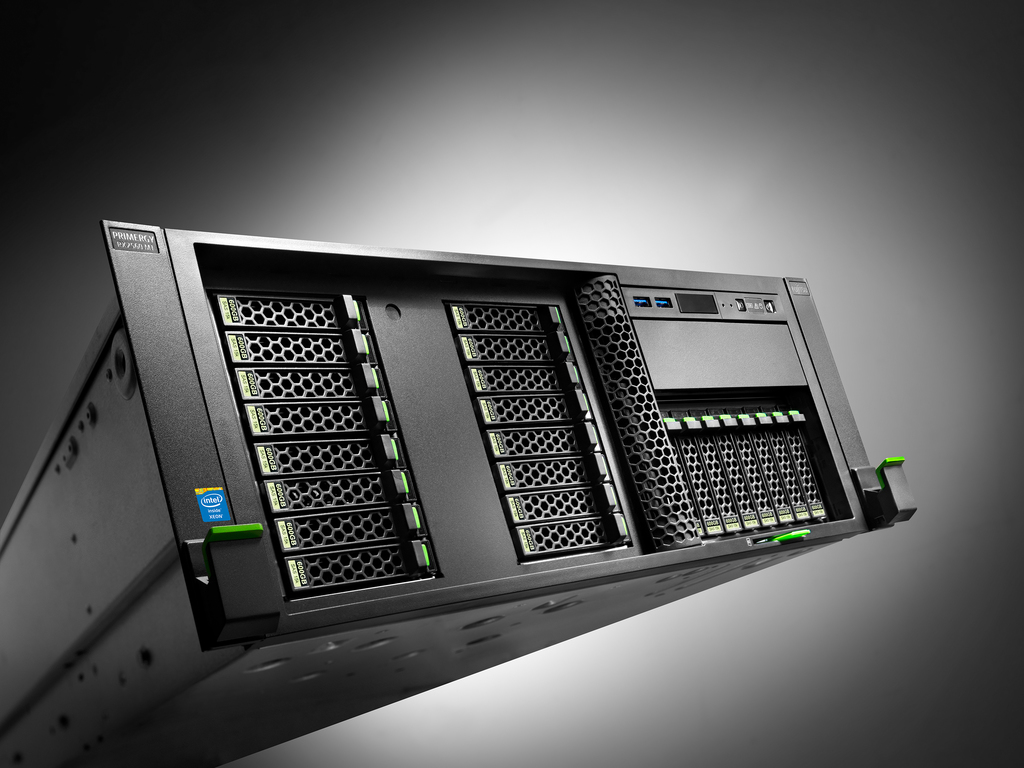
\includegraphics[height=\paperheight]{RX2560-M1.jpg}};
}

\begin{frame} 
  \titlepage 
\end{frame} 

\usebackgroundtemplate{} %unset

\begin{frame}{Table of content}
  \tableofcontents
  % You might wish to add the option [pausesections]
\end{frame}


\section{Fujitsu Primergy servers family}
  \subsection{What is iRMC}
  \subsection{Software - ServerView Suite}
  \subsection{iRMC Firmware}
  \subsection{Open standarts: IPMI protocol and others}
  \subsection{Demo: WebIF and IPMI}

\section{From iRMC S1 on ThreadX to iRMC S4 on Linux}
  \subsection{Early ages - ThreadX : S1 - S3}
  \subsection{Migration to Linux: S4}
  \subsection{Demo: RemoteManager - bug-to-bug compatible}

\section{Linux based firmware}
  \subsection{Components}
  \subsection{Mixing FOSS and propiertary code}
  \subsection{Develoment environment}
  \subsection{Where is the sources?}
  \subsection{Demo: inside the Linux on iRMC}


%
\begin{frame} 
  \titlepage 
\end{frame} 

\begin{frame}{Disclaimer}
  \Large{Неофициальное содержание:}
  \begin{itemize}
    \item \normalsize{расисткие сплетни о коммерческих вендорах}
    \item анальное огораживание частных недо-серверов 
    \item убедительное обоснование пионерских поделок
    \item неприкрытая реклама side-проекта MLUG
  \end{itemize}


  \emph{ }\newline \pause

  Автор доклада гарантирует эмоционально окрашенные субьективные оценки.
\end{frame}

\begin{frame}{Краткое содержание, официально}
  \tableofcontents
  % You might wish to add the option [pausesections]
\end{frame}

\section{Технология XMPP/Jabber}

\begin{frame}{Общие сведения}
  \Large{«Православие,\\Самодержавие,\\Народность»} 
\end{frame}

\begin{frame}{Общие сведения}
  \Large{ \sout{«Православие,\\Самодержавие,\\Народность»} }

  «Открытые протоколы,\\ Децентрализация,\\Instant Messaging and Presence»

\end{frame}

\begin{frame}{Основа - протокол}
  \begin{itemize}
    \item Протокол XMPP\footnote{Extensible Messaging and Presence Protocol}

    \item Внутри XML

    \item Стандартизирован IETF\footnote{RFC 6120, RFC 6121, и RFC 6122}.

    \item Доп расширения к RFC: XEP \footnote{ ``XMPP Standarts Foundation``}
  \end{itemize}

\end{frame}

\begin{frame}{Что умеет XMPP}
  С т.ч. рядового пользователя:
  \begin{itemize}
    \item обычные и групповые чаты
    \item передача голоса и видео
    \item передача файлов
    \item серверная история
    \item одновременное подключение нескольких клиентов
  \end{itemize}
\end{frame}

\begin{frame}{Как выглядит (Psi)}
  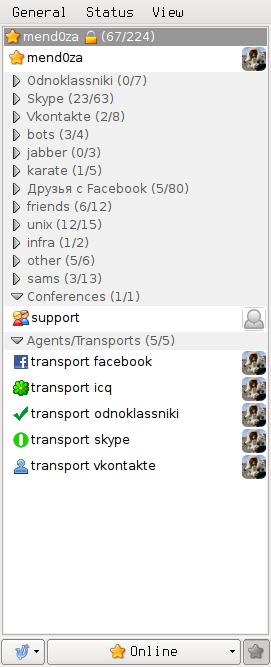
\includegraphics[height=5.9cm]{psi-plus}\emph{ }
  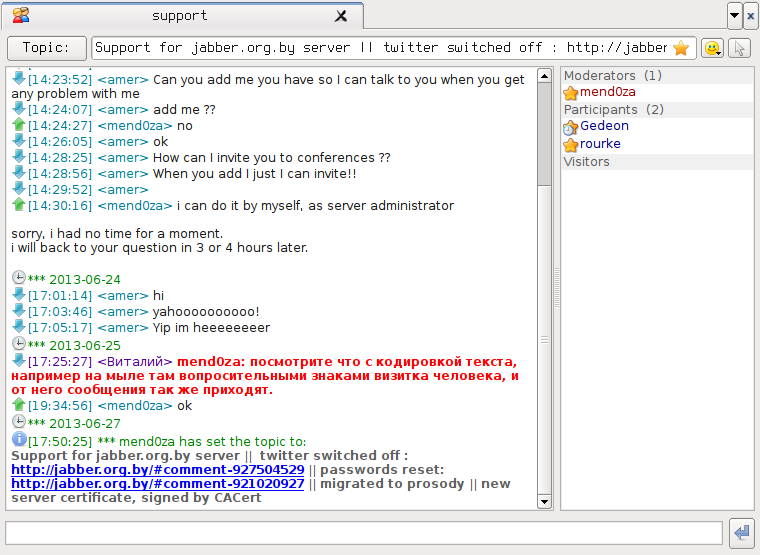
\includegraphics[height=5.9cm]{muc}
  % 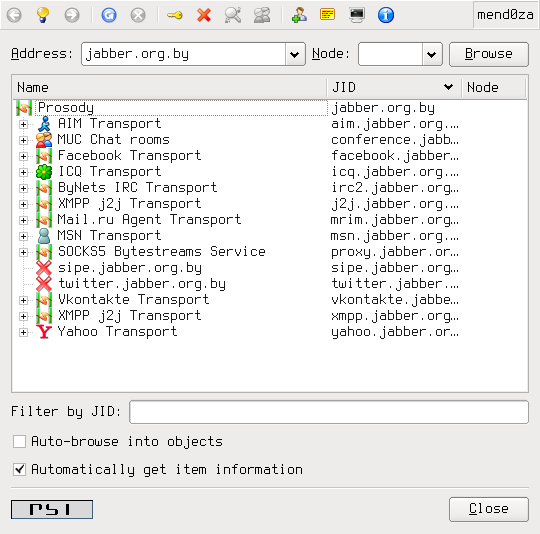
\includegraphics[height=4cm]{discovery}
\end{frame}

\begin{frame}{Базовые понятия и функции}

  \begin{block}{JID : login@server}
    Каждый сервер - независимая сущность. 

    Сервера договариваются между собой по XMPP.

    XMPP Federation или XMPP s2s.
  \end{block} \pause

  \begin{block}{Публикация статуса и подписка на него}
    Примеры: 
    \begin{enumerate}
      \item статус контакта (в сети | away | n/a)
      \item какую музыку слушает
      \item подписка на ботов (погода, новости, etc)
    \end{enumerate}
  \end{block}

\end{frame}


\begin{frame}{Наиболее интересные возможности}
  \begin{itemize}
    \item серверные шлюзы (транспорты) в другие IM\footnote{ICQ, Skype, MSN, SIP, IRC, Email, в том числе и другие XMPP}
    \item шифрование: клиент-сервер и сервер-сервер\footnote{плюс можно шифровать открывать открытым ключом}
    \item удалённая передача команд
    \item инструменты совместной работы\footnote{Abiword, Inkskape, LibreOffice, Coccinella}
    \item микроблоггинг
    \item сетевые распределённые игры
    \item geolocation
    \item cервисы авторизации: OpenID, OAuth
    \item облачные вычисления
  \end{itemize}

\end{frame}


%\section{XMPP против других IM}

\subsection{Подъём и падение XMPP}
\begin{frame}{Подъём \ldots и падение XMPP}
  \begin{block}{Подъём}
    Технология XMPP заняла свои позиции. \\
    Сервисы: Facebook, GTalk, VKontakte, WhatsApp. \\
    Бизнес-решения: MS Lync, Cisco Unified Presence.

    Позволяют подключится по XMPP или основаны на нём
  \end{block} \pause

  \begin{block}{\ldots и падение}
    Разработчики корпоративных и открытых решений множат мало функциональные и/или несовместимые решения.
  \end{block}
\end{frame}

\begin{frame}{Метнём коричневые комки правды}
  \begin{block}{Серверные красавчики}
    \begin{itemize}
      \item Отключен s2s : Facebook, Vkontakte, Odnoklassniki
      \item Нельзя поменять VCard : почти все
      \item Странное поведение серверов: Google Talk
      \item Нет server-side history
      \item Нет поддержки групп : см s2s
    \end{itemize} 
  \end{block}\pause

  \begin{block}{Клиентские красавчики}
    \begin{itemize}
      \item нет поддержки Service Discovery (imo, im+, xabber)
      \item нет поддержки multi user chat
      \item нет групп в ростере (imo)
    \end{itemize}
    Особенно мало умеют многопротокольные клиенты\footnote{где XMPP лишь одна из опций}.
  \end{block}
\end{frame}

\begin{frame}{Итого}
  \begin{block}{Теоретическое богатство возможностей XMPP}
  \end{block}

  \pause

  \begin{block}{\ldots недоступно в качественном коробочном продукте.}
  \end{block}

  \pause

  \begin{block}{Часто требует ощутимых усилий от оператора сервера \ldots}
  \end{block}
  
  \pause

  \begin{block}{или даже от конечного пользователя \ldots}
  \end{block}
\end{frame}

\subsection{Заметки о войнах IM}

\begin{frame}{1я Мировая Война IM}
    \alert{Время}: от конца 90-х до (приблизительно) 2005. 

    \alert{Предпосылки}: Широкое распространение Internet. Dial-Up. 
    
    \alert{Начало}: Появился ICQ. 
      
    \alert{Ключевой функционал}: передача текста, сообщения и групповые чаты

    \alert{Кто?}: ICQ, AIM, MSN, Yahoo, IRC

    \alert{Конец войны}: интеграция протоколов и клиентов
\end{frame}

\begin{frame}{Подходы к IM Protocol Hell}
  2 магистральных подхода, cформировались в ходе 1й Войны:

  \begin{block}{Многопротокольные клиенты}
    Miranda, Pidgin, Trillian, Empathy/Telepathy
  \end{block}

  \pause

  \begin{block}{Сервер-интегратор}
    Клиент работает по 1 протоколу. 
    
    Сервер транслирует протоколы в 1.

    Известные реализации: XMPP/Jabber, MS Lync, imo.im, Cisco Unified Meeting Place
  \end{block}

\end{frame}

\begin{frame}{Jabber/XMPP - way}
  \begin{itemize}
    \item Реверс-инжениринг закрытых протоколов
    \item Написаны транспорты ко всем известным протоколам
  \end{itemize}
\end{frame}

\begin{frame}{2я Мировая Война IM}
    \alert{Время}:  2005. 

    \alert{Предпосылки}: Широкополосный скоростной интернет
    
    \alert{Начало}: Появился Skype. 
      
    \alert{Ключевой функционал}: голосовые и видео-звонки

    \alert{Кто?}: Skype, WhatsApp, Google Hangout, Viber, SIP

    \alert{Конец войны}: продолжается
\end{frame}

{
\usebackgroundtemplate{
\includegraphics[width=\paperwidth,height=\paperheight]{goryaschii_tank_u_reki}}
\begin{frame}{Репортаж из горящего танка\footnote{\alert{Hint: внутри WoT Chat - Jabber}}}

  \alert{
    \begin{enumerate}
      \item Cтеки протоколов и технологий: SIP\footnote{\alert{Skype, Viber}} и XMPP\footnote{\alert{WhatsApp}}

      \item Полностью закрытые решения без внешнего API

      \item Производитель воспринимает своих пользователей как свою собственность 

    \end{enumerate}
  }

\end{frame}
}

{
\usebackgroundtemplate{
\includegraphics[width=\paperwidth,height=\paperheight]{facebook-logo}}
\begin{frame}{Анальное огораживание, Facebook-way}
  \begin{block}{Есть}
    \begin{enumerate}
      \item чат с пользователями в Facebook
      \item публикация статуса онлайн/оффлайн
      \item несколько соединений одновременно
    \end{enumerate}
  \end{block} 
  \pause

  \begin{block}{Нет / Не работает}
    \begin{enumerate}
      \item S2S
      \item сервисов и транспортов
      \item групп и управления группами
      \item видео и аудио
      \item не работает VCard 
      \item запутанная схема подключения
      \item нельзя публиковать и читать материалы в ленте
      \item нельзя подключать новых пользователей
    \end{enumerate}
  \end{block}
\end{frame}
}

{
\usebackgroundtemplate{
\includegraphics[width=\paperwidth,height=\paperheight]{google-talk-logo}}
\begin{frame}{Былинный отказ: Google Talk}
  \alert{Whats going on? Факты.}

  \begin{itemize}
    \item с 2006 до 2013 - GTalk стал крупнейшим сервером XMPP/Jabber
    \item \alert{ТОЛЬКО} за счёт навязывания Google Talk в нагрузку к GMail и Android\footnote{см словарь - ``Связанная покупка''}. \pause
    \item Голос, видео и звонки на телефон - позже чем в скайп
    \item реализация - слабо совместима с остальным XMPP \pause
    \item Google не замечен в работе над стандартами XMPP
    \item Единственный вклад - Jingle и GSoC
  \end{itemize}
  \pause
  \alert{Вывод: компания сильно не вкладывалась в XMPP, и выбросила его без сожаления. Вслед за RSS Reader}

\end{frame}
}


%\section{Community-driven XMPP сервер}

\begin{frame}{Зачем нужны community XMPP/Jabber сервера}
  
\includegraphics[height=3cm]{jabber-logo}
  \begin{itemize}
    \item Коммерческие поставщики ограничены т.н. ``выгодным''
    \item От набора заготовок к коробочному продукту
    \item Сокращение дистанции между пользователями и участниками создания
    \item Влияем на результат, не покупая целиком Google, Viber или Facebook
    \item Инновации: передний край технологии XMPP
    \item Повышение устойчивости экосистемы XMPP
  \end{itemize}
\end{frame}

\begin{frame}{Классический Community-проект}

  Сервер jabber.org.by возник и базируется на кадрах из белорусского FOSS-community\footnote{side-проект "Minsk Linux Users Group" и сообщества вокруг Linux.by"}.

  "Собор и Базар" by ESR:
  \begin{itemize}
    \item операторы пользуются сами большей частью функционала
    \item стараются делать, что просят пользователи\footnote{даже если им самим запрошенные функции не нужны}
    \item пользователи привлекаются к тестированию и улучшению  сервисов
    \item по мере сил взаимодействовуют с upstream (spectrum, pyicqt)
    \item время от времени смена личного состава
  \end{itemize}
\end{frame}

%\section{Ceрвер jabber.org.by/jabber.linux.by}
\begin{frame}{О сервере}
  Первый, и единственный публичный сервер в РБ.

  Особенности:
  \begin{itemize}
      \item открытая регистрация
      \item community-driven
      \item широкий набор транспортов\footnote{ICQ, MSN, AIM, Yahoo, Twitter, MRIM и несколько транспортов в XMPP под разными именами}
      \item физически расположен в Беларуси \footnote{провайдер BASNET} 
  \end{itemize}

  Опыт поддержки и эксплуатации указанного сервера в течении 9 лет и положен в основу доклада.
\end{frame}

\begin{frame}{Hardware und Software}

  \begin{block}{Hardware} 
    \begin{itemize}
      \item Контейнер в OpenVZ
      \item RAM 2GB\footnote{до 4GB если другие контейнеры не требуют}  
      \item 40 GB HDD
      \item Intel(R) Xeon(R) CPU E5506  @ 2.13GHz  
    \end{itemize} 
  \end{block}
 
  \pause
  
  \begin{block}{Software}
    \begin{itemize}
      \item Debian GNU/Linux 7.x (stable)
      \item jabberd: Prosody 0.9
      \item транспорты Spectrum2
    \end{itemize}
  \end{block}
\end{frame}

\subsection{Вехи развития jabber.org.by}

\begin{frame}{Начало}
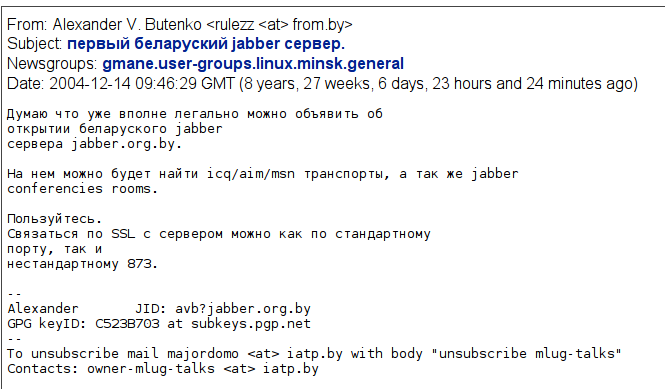
\includegraphics[width=10cm]{beginning}
\end{frame}

\begin{frame}{События}

  \begin{itemize}
    \item 14 декабря 2004 года. Запуск.
    \item конец 2005. Пользователи (cymrak, booxter, trenka) по своей инициативе собирают деньги и апгрейдят сервер.
    \item 14.12.2006 Внутренний hackaton по исправлению утечек памяти в PyICQt.  
    \item 09.03.2007. Эмиграция MrDeath в Доминиканскую Республику
    \item март 2008. Остановка сервиса и далее переезд на FreeBSD
    \item август 2009. тестированиe под нагрузкой и исправлении утечки памяти в PyICQt 0.8.1.5
    \item февраль 2011. Переезд на Debian 6.x/OpenVZ. Переход на сервисы Spectrum.
    \item сентябрь 2012-май 2013. Эпическая Борьба с сирийскими ботами.
    \item июнь 2013. Потеря пользовательских паролей (неудачный апдейт)
    \item 14 июня 2013. Переход на Prosody.
  \end{itemize}

\end{frame}

\begin{frame}{MrDeath: Привет из Доминиканы - 1}
  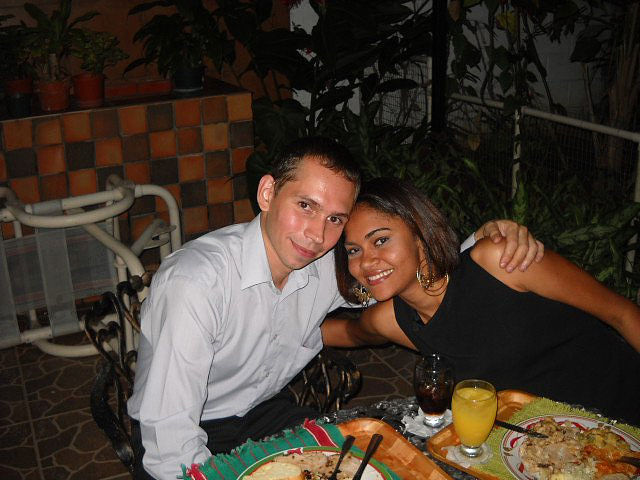
\includegraphics[width=10cm]{avb_with_Karla}
\end{frame}

\begin{frame}{MrDeath: Привет из Доминиканы - 2}
  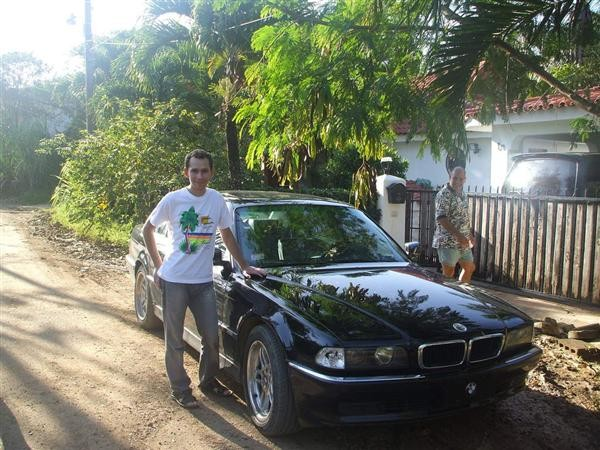
\includegraphics[width=10cm]{avb_with_black_boomer}
\end{frame}

\begin{frame}{Текущий статус сервера}
   \begin{itemize}
      \item учётки @jabber.org.by и @jabber.linux.by
      \item ~ 50-70 активных пользователей
      \item S2S - 130-150 одновременно
      \item транспорты - до 400 юзеров одновременно
    \end{itemize}
\end{frame}





\section*{Summary}
\begin{frame}{Questions? Remarks?}
  
  \begin{center}
    \pgfuseimage{fujitsu-shaping}
  \end{center}

  \normalsize{Fujitsu Primergy servers: http://www.fujitsu.com/fts/products/computing/servers/primergy/ }
  \normalsize{iRMC S4 manual: http://manuals.ts.fujitsu.com/file/11470/irmc-s4-ug-en.pdf}
  
  \normalsize{Fujitsu Technology Solutions: http://www.fujitsu.com/fts}

  contact: Vladimir.Shakhov at ts.fujitsu.com


\end{frame}

\end{document}
